\chapter{Datasets and Monte Carlo Simulations}

\section{Data}

\subsection{Triggers and Datasets}
\label{sec:trigpaths}

This analysis uses a data sample recorded by the CMS experiment during 2016, corresponding to $\usedLumi$ of data. 
The datasets are listed in Table~\ref{tab:datasets_data}, along with the integrated luminosity.  
The analysis relies on five different primary datasets (PDs), 
{\it DoubleEG}, {\it DoubleMuon}, {\it MuEG}, {\it SingleElectron}, and {\it SingleMuon},
each of which combines a certain collection of HLT paths. 
To avoid duplicate events from different primary datasets, events are taken:
\begin{itemize}
\item from DoubleEG if they pass the diEle or triEle triggers,
\item from DoubleMuon if they pass the diMuon or triMuon triggers and fail the diEle and triEle triggers,
\item from MuEG if they pass the MuEle or MuDiEle or DiMuEle triggers and fail the diEle, triEle, diMuon and triMuon triggers,
\item from SingleElectron if they pass the singleElectron trigger and fail all the above triggers. 
\item from SingleMuon if they pass the singleMuon trigger and fail all the above triggers. 
\end{itemize} 

The HLT paths used for 2016 collision data are listed in Table~\ref{tab:triggerPaths}, 
together with their L1 seed, prescale value and the associated primary dataset.

%The JSON files are the following:
%\begin{itemize}
%\item Cert\_13TeV\_16Dec2015ReReco\_Collisions15\_50ns\_JSON.txt (for 50 ns data),
%\item Cert\_13TeV\_16Dec2015ReReco\_Collisions15\_25ns\_JSON\_Silver.txt (for 25 ns data).
%\end{itemize} 

\begin{table}[h]
\tiny
    \centering
    \begin{tabular}{|l|l|l|} 
\hline %----------------------------------------------------------------------------------------
\hline %---------------------------------------------------------------------------------------- 
Run-range & Dataset & Integrated luminosity \\
\hline %----------------------------------------------------------------------------------------
\hline %---------------------------------------------------------------------------------------- 
\multirow{5}{*}{273150-275376} & /DoubleMuon/Run2016B-23Sep2016-v3/AOD &  \multirow{5}{*}{$5.892\ \text{fb}^{-1}$} \\ 
& /DoubleEG/Run2016B-23Sep2016-v3/AOD &  \\ 
& /MuonEG/Run2016B-23Sep2016-v3/AOD &  \\ 
& /SingleElectron/Run2016B-23Sep2016-v3/AOD &  \\ 
& /SingleMuon/Run2016B-23Sep2016-v3/AOD &  \\ 
\hline
\multirow{5}{*}{275656-276283} & /DoubleMuon/Run2016C-23Sep2016-v1/AOD &  \multirow{5}{*}{$2.646\ \text{fb}^{-1}$}  \\ 
& /DoubleEG/Run2016C-23Sep2016-v1/AOD &  \\ 
& /MuonEG/Run2016C-23Sep2016-v1/AOD &  \\ 
& /SingleElectron/Run2016C-23Sep2016-v1/AOD &  \\ 
& /SingleMuon/Run2016C-23Sep2016-v1/AOD &  \\ 
\hline
\multirow{5}{*}{276315-276811} & /DoubleMuon/Run2016D-23Sep2016-v1/AOD &  \multirow{5}{*}{$4.353\ \text{fb}^{-1}$} \\ 
& /DoubleEG/Run2016D-23Sep2016-v1/AOD &  \\ 
& /MuonEG/Run2016D-23Sep2016-v1/AOD &  \\ 
& /SingleElectron/Run2016D-23Sep2016-v1/AOD &  \\ 
& /SingleMuon/Run2016D-23Sep2016-v1/AOD &  \\ 
\hline
\multirow{5}{*}{276831-277420} & /DoubleMuon/Run2016E-23Sep2016-v1/AOD &  \multirow{5}{*}{$4.117\ \text{fb}^{-1}$} \\ 
& /DoubleEG/Run2016E-23Sep2016-v1/AOD &  \\ 
& /MuonEG/Run2016E-23Sep2016-v1/AOD &  \\ 
& /SingleElectron/Run2016E-23Sep2016-v1/AOD &  \\ 
& /SingleMuon/Run2016E-23Sep2016-v1/AOD &  \\ 
\hline
\multirow{5}{*}{277932-278808} & /DoubleMuon/Run2016F-23Sep2016-v1/AOD &  \multirow{5}{*}{$3.186\ \text{fb}^{-1}$} \\ 
& /DoubleEG/Run2016F-23Sep2016-v1/AOD &  \\ 
& /MuonEG/Run2016F-23Sep2016-v1/AOD &  \\ 
& /SingleElectron/Run2016F-23Sep2016-v1/AOD &  \\ 
& /SingleMuon/Run2016F-23Sep2016-v1/AOD &  \\ 
\hline
\multirow{5}{*}{278820-280385} & /DoubleMuon/Run2016G-23Sep2016-v1/AOD &  \multirow{5}{*}{$7.721\ \text{fb}^{-1}$} \\ 
& /DoubleEG/Run2016G-23Sep2016-v1/AOD &  \\ 
& /MuonEG/Run2016G-23Sep2016-v1/AOD &  \\ 
& /SingleElectron/Run2016G-23Sep2016-v1/AOD &  \\ 
& /SingleMuon/Run2016G-23Sep2016-v1/AOD &  \\ 
\hline
\multirow{15}{*}{281207-284068} & /DoubleMuon/Run2016H-PromptReco-v1/AOD &  \multirow{15}{*}{$8.857\ \text{fb}^{-1}$} \\ 
& /DoubleEG/Run2016H-PromptReco-v1/AOD &  \\ 
& /MuonEG/Run2016H-PromptReco-v1/AOD &  \\ 
& /SingleElectron/Run2016H-PromptReco-v1/AOD &  \\ 
& /SingleMuon/Run2016H-PromptReco-v1/AOD &  \\ 
& /DoubleMuon/Run2016H-PromptReco-v2/AOD &  \\ 
& /DoubleEG/Run2016H-PromptReco-v2/AOD &  \\ 
& /MuonEG/Run2016H-PromptReco-v2/AOD &  \\ 
& /SingleElectron/Run2016H-PromptReco-v2/AOD &  \\ 
& /SingleMuon/Run2016H-PromptReco-v2/AOD &  \\ 
& /DoubleMuon/Run2016H-PromptReco-v3/AOD &  \\ 
& /DoubleEG/Run2016H-PromptReco-v3/AOD &  \\ 
& /MuonEG/Run2016H-PromptReco-v3/AOD &  \\ 
& /SingleElectron/Run2016H-PromptReco-v3/AOD &  \\ 
& /SingleMuon/Run2016H-PromptReco-v3/AOD &  \\ 
\hline %----------------------------------------------------------------------------------------
\hline %----------------------------------------------------------------------------------------
     \end{tabular}
%\small
    \caption{ Datasets used in the analysis. }
    \label{tab:datasets_data}
\end{table}


\begin{table}[h]
\tiny
    \centering
    \begin{tabular}{|l|l|c|l|} 
\hline %--------------------------------------------------------------------------------------------------------------------------
HLT path                      				       & L1 seed                          & prescale  & primary dataset \\
\hline %--------------------------------------------------------------------------------------------------------------------------
\verb| HLT_Ele17_Ele12_CaloIdL_TrackIdL_IsoVL_DZ       | & \verb| L1_DoubleEG_15_10    |  & 1 & DoubleEG \\
\verb| HLT_Ele23_Ele12_CaloIdL_TrackIdL_IsoVL_DZ       | & \verb| L1_DoubleEG_22_10    |  & 1 & DoubleEG \\
\verb| HLT_DoubleEle33_CaloIdL_GsfTrkIdVL              | & \verb| (Multiple)           |  & 1 & DoubleEG \\
\verb| HLT_Ele16_Ele12_Ele8_CaloIdL_TrackIdL           | & \verb| L1_TripleEG_14_10_8  |  & 1 & DoubleEG \\
\verb| HLT_Mu17_TrkIsoVVL_Mu8_TrkIsoVVL                | & \verb| L1_DoubleMu_11_4     |  & 1 & DoubleMuon \\
\verb| HLT_Mu17_TrkIsoVVL_TkMu8_TrkIsoVVL              | & \verb| L1_DoubleMu_11_4     |  & 1 & DoubleMuon \\
\verb| HLT_TripleMu_12_10_5                            | & \verb| L1_TripleMu_5_5_3    |  & 1 & DoubleMuon \\
\verb| HLT_Mu8_TrkIsoVVL_Ele17_CaloIdL_TrackIdL_IsoVL  | & \verb| L1_Mu5_EG15          |  & 1 & MuonEG \\
\verb| HLT_Mu8_TrkIsoVVL_Ele23_CaloIdL_TrackIdL_IsoVL  | & \verb| L1_Mu5_EG20          |  & 1 & MuonEG \\
\verb| HLT_Mu17_TrkIsoVVL_Ele12_CaloIdL_TrackIdL_IsoVL | & \verb| L1_Mu12_EG10         |  & 1 & MuonEG \\
\verb| HLT_Mu23_TrkIsoVVL_Ele12_CaloIdL_TrackIdL_IsoVL | & \verb| L1_Mu20_EG10         |  & 1 & MuonEG \\
\verb| HLT_Mu23_TrkIsoVVL_Ele8_CaloIdL_TrackIdL_IsoVL  | & \verb| L1_SingleMu*         |  & 1 & MuonEG \\
\verb| HLT_Mu8_DiEle12_CaloIdL_TrackIdL                | & \verb| L1_Mu6_DoubleEG10    |  & 1 & MuonEG \\
\verb| HLT_DiMu9_Ele9_CaloIdL_TrackIdL                 | & \verb| L1_DoubleMu7_EG7     |  & 1 & MuonEG \\
\verb| HLT_Ele25_eta2p1_WPTight                        | & \verb| L1_SingleEG*         |  & 1 & SingleElectron \\
\verb| HLT_Ele27_WPTight                               | & \verb| L1_SingleEG*         |  & 1 & SingleElectron \\
\verb| HLT_Ele27_eta2p1_WPLoose_Gsf                    | & \verb| L1_SingleEG*         |  & 1 & SingleElectron \\
\verb| HLT_IsoMu20 OR HLT_IsoTkMu20                    | & \verb| L1_SingleMu*         |  & 1 & SingleMuon \\
\verb| HLT_IsoMu22 OR HLT_IsoTkMu22                    | & \verb| L1_SingleMu*         |  & 1 & SingleMuon \\
\hline %--------------------------------------------------------------------------------------------------------------------------
    \end{tabular}
%\small
    \caption{Trigger paths used in 2016 collision data.}
    \label{tab:triggerPaths}
\end{table}


\subsection{Trigger Efficiency}

The efficiency in data of the combination of triggers used in the anlysis with respect to the offline reconstruction and selection is measured
by considering 4$\ell$ events triggered by single lepton triggers. One of the four reconstructed leptons ( the ``tag'') is geometrically matched 
to a trigger object passing the final filter of one of the single muon or single electron triggers. The other three leptons are 
used as ``probes''. In each 4$\ell$ event there are up to 4 possible tag-probe combinations, and all possible combinations are counted in the
denominator of the efficiency. For each of the three probe leptons all matching trigger filter objects are collected. Then the matched trigger filter
objects of the three probe leptons are combined in attempt to reconstruct any of the triggers used in the anlysis. If any of the analysis triggers
can be formed using the probe leptons, the set of probes is also counted in the numerator of the efficiency.

This method does not have a perfect closure in MC events due to the fact that the presence of a fourth lepton increases the trigger efficiency,
and this effect is not accounted for. Also, in the  $2e2\mu$ final state, the three probe leptons cannot be combined to form all possible triggers which 
can collect events with two electrons and two muons (e.g. if the tag lepton is an electron, the three remaining leptons cannot pass a double electron
trigger). Therefore the method is also exercised on MC and the difference between data and MC is used to determine the reliability of the simulation.
 The efficiency plotted as a function of the minimum $p_{\rm{T}}$ of the three probe leptons in data and MC using this method can be seen in 
Fig.\ref{fig:TrigEff}. The MC efficiency describes well the data within the statistical uncertainties.

%=======
\begin{figure}[!htb]
\vspace*{0.3cm}
\begin{center}
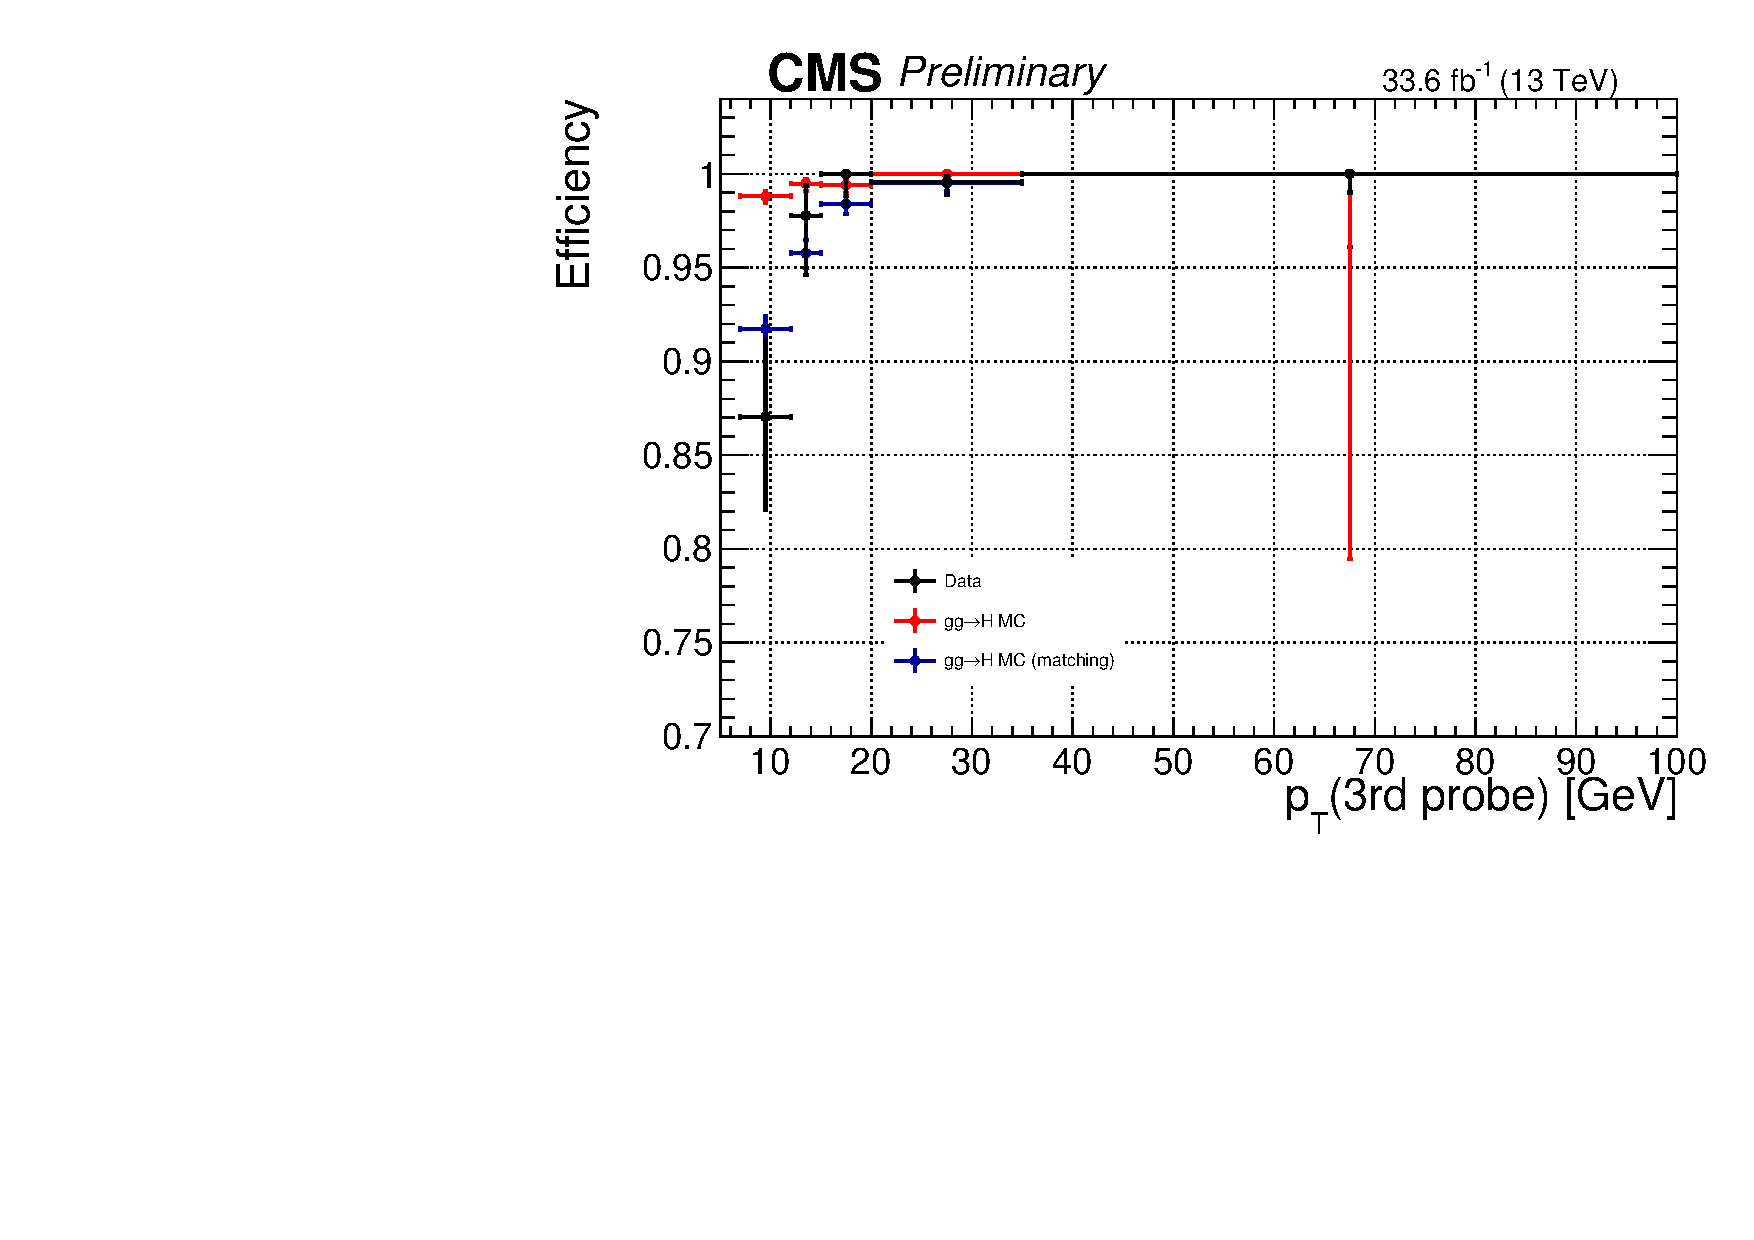
\includegraphics[width=0.45\textwidth]{Figures/Trigger/Histo_TrigEff_ptMin_4e.pdf} 
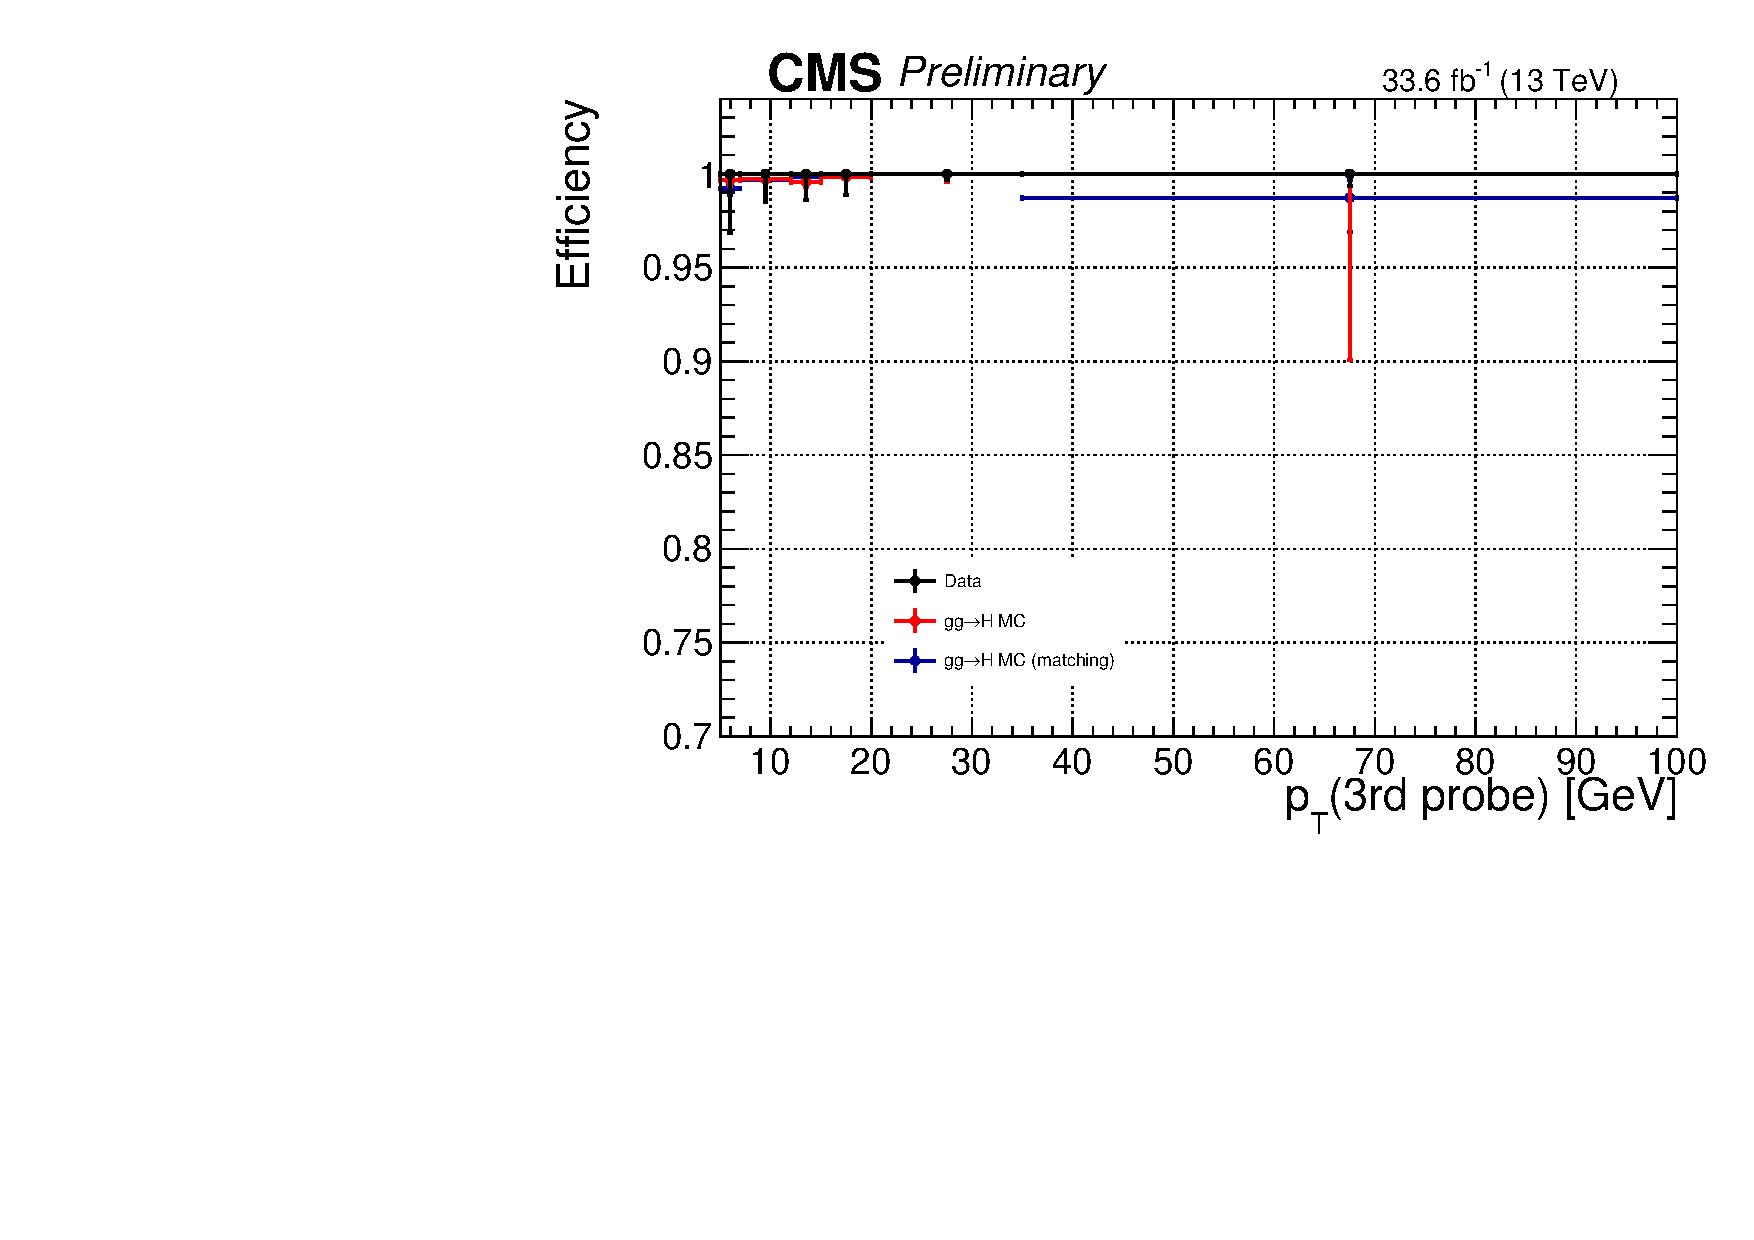
\includegraphics[width=0.45\textwidth]{Figures/Trigger/Histo_TrigEff_ptMin_4mu.pdf} \\
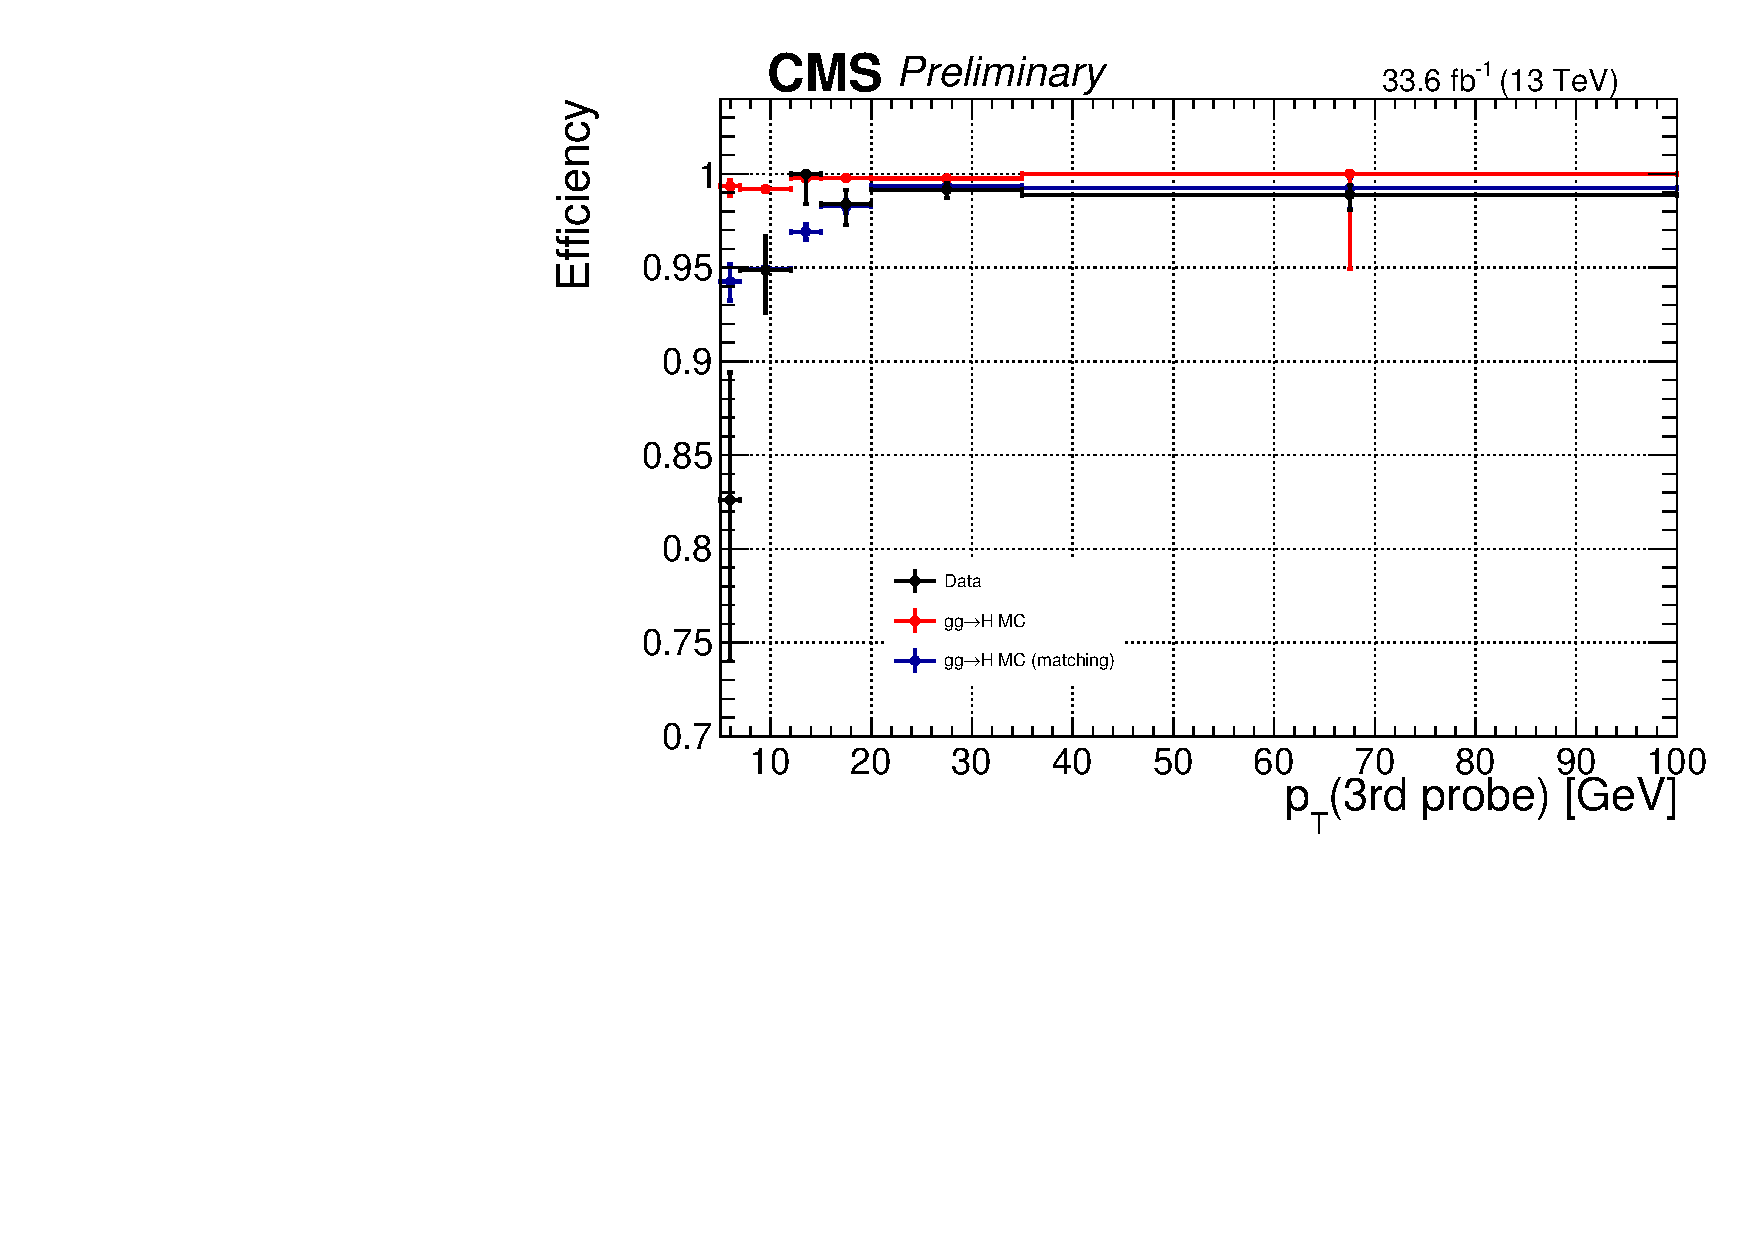
\includegraphics[width=0.45\textwidth]{Figures/Trigger/Histo_TrigEff_ptMin_2e2mu.pdf} 
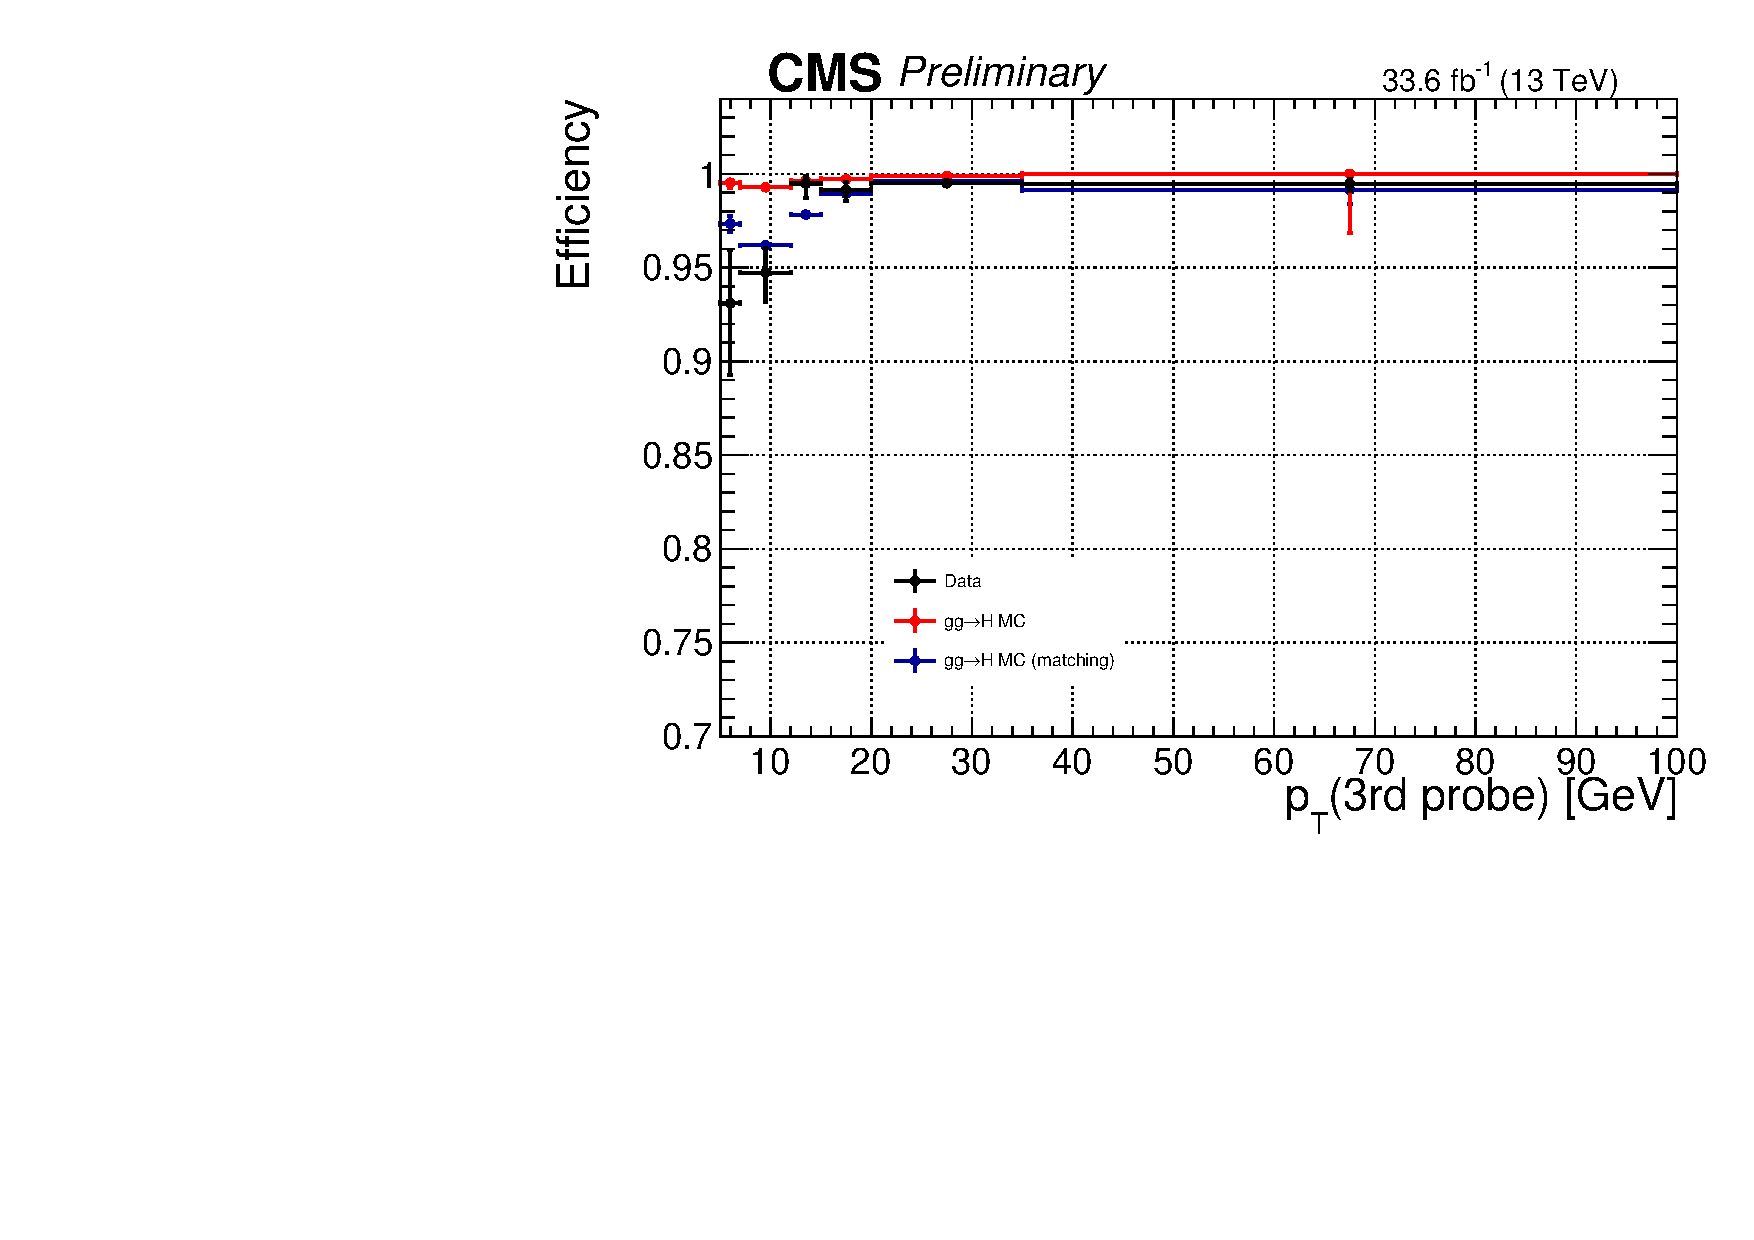
\includegraphics[width=0.45\textwidth]{Figures/Trigger/Histo_TrigEff_ptMin_4l.pdf} \\
\caption{Trigger efficiency measured in data using $4\ell$ events collected by single lepton triggers for the $4e$ (top left), $4\mu$ (top right), $2e2\mu$ (bottom left) and $4\ell$ (bottom right) final states. 
\label{fig:TrigEff}}
\end{center}
\end{figure}
%=======

A summary of the trigger efficiencies in MC truth, and in MC and data using the tag and probe method are summarized in table~\ref{tab:TrigEff}. The trigger
efficiency in simulation is found to be $>99\%$ in each final state.

\begin{table}[h]
    \centering
    \begin{tabular}{|c|c|c|c|c|} 
\hline %----------------------------------------------------------------
Final State  & $\ggH$ MC & $\ggH$ MC (matching)  & Data (matching)   \\
\hline %----------------------------------------------------------------
$4e$  & 0.991$^{+.002}_{-0.002}$ & 0.948$^{+.004}_{-0.004}$ & 0.982$^{+.005}_{-0.007}$ \\
$4\mu$  & 0.997$^{+.001}_{-0.001}$ & 0.997$^{+.001}_{-0.001}$ & 1.000$^{+.000}_{-0.001}$ \\
$2e2\mu$  & 0.995$^{+.001}_{-0.001}$ & 0.964$^{+.002}_{-0.002}$ & 0.983$^{+.003}_{-0.004}$ \\
\hline %----------------------------------------------------------------
    \end{tabular}
    \caption{Trigger efficiencies measured using $4\ell$ events.}
    \label{tab:TrigEff}
\end{table}

\section{Simulation}

\subsection{Signal Samples}

The signal samples used are centrally produced for the benchmarks defined in the previous section and are summarized in Table~\ref{tab:sig}.

\begin{table}
\resizebox{\textwidth}{!}{%
\begin{tabular}{| l | l |}
\hline
Dataset & Parameters\\
\hline
/ZprimeToA0hToA0chichihZZTo4l\_2HDM\_MZp-*\_MA0-300\_13TeV-madgraph-pythia8/[1] & $m_{A^0} = $ 300 GeV \\
/ZprimeToA0hToA0chichihZZTo4l\_2HDM\_MZp-*\_MA0-*\_13TeV-madgraph/[2] & $m_{A^0} \neq $ 300 GeV \\
/MonoHZZ4l\_ZpBaryonic\_MZp-*\_MChi-*\_13TeV-madgraph/[3] & \\
\hline
$[1]$ RunIISpring16DR80-premix\_withHLT\_80X\_mcRun2\_asymptotic\_v14-v1/AODSIM & \\
$[2]$ RunIISpring16reHLT80-PUSpring16RAWAODSIM\_reHLT\_80X\_mcRun2\_asymptotic\_v14-v1/AODSIM & \\
$[3]$ RunIISpring16DR80-premix\_withHLT\_80X\_mcRun2\_asymptotic\_v14-v1/AODSIM & \\
\hline
\end{tabular}}
\caption{Benchmark signal samples analyzed.}\label{tab:sig}
\end{table}

\subsection{Background Samples}

Descriptions of the SM Higgs boson production are obtained using the 
{\sc powheg V2}~\cite{Alioli:2008gx,Nason:2004rx,Frixione:2007vw} generator for the five main production modes: 
gluon fusion ($\ggH$) including quark mass effects~\cite{Bagnaschi:2011tu}, vector boson fusion 
(VBF)~\cite{Nason:2009ai}, and associated production (WH, $\cPZ$H and \ttbar$\,$H~\cite{Hartanto:2015uka}). 
In the case of WH and $\cPZ$H the {\sc MiNLO HVJ} extension of {\sc powheg} is used~\cite{Luisoni:2013kna}. 
The description of the decay of the Higgs boson to four leptons is obtained using the {\sc JHUgen} 
generator~\cite{Gao:2010qx}. In the case of WH, $\cPZ$H and \ttbar$\,$H, the Higgs boson is allowed
to decay to H$\to \cPZ \cPZ \to 2\ell2$X such that 4-lepton events where two leptons originate from 
the decay of associated $\cPZ$, W bosons or top quarks are also taken into account in the simulation. 
Showering of parton-level events is done using {\sc pythia8.209}, and in all cases matching is performed by 
allowing QCD emissions at all energies in the shower and vetoing them afterwards according to the 
{\sc powheg} internal scale. All samples are generated with the NNPDF 3.0 NLO parton distribution 
functions (PDFs)~\cite{Ball:2014uwa}. The list of Higgs signal samples and their cross sections are shown in 
Table~\ref{tab:SignalSamples}.

\begin{table}
\begin{scriptsize}
    \centering
\resizebox{\textwidth}{!}{%
    \begin{tabular}{|l|l|r|}
   \hline
 Process & Dataset Name & $\sigma\times BR (\times\epsilon_{\text{filter}})$ \\ \hline
 $\rm{gg}\to\rm{H}\to\cPZ\cPZ \to 4\ell$ & /GluGluHToZZTo4L\_M125\_13TeV\_powheg2\_JHUgenV6\_pythia8 & $12.18~\rm{fb}$ \\ % & $12.12~\rm{fb}$ \\
 $\rm{qq}\to\rm{Hqq}\to\cPZ\cPZ\rm{qq}\to4\ell qq$ & /VBF\_HToZZTo4L\_M125\_13TeV\_powheg2\_JHUgenV6\_pythia8 & $1.044~\rm{fb}$ \\ % $1.034~\rm{fb}$ \\
 $\rm{q\bar{q}}\to\rm{W^{+}H}\to\rm{W^{+}}\cPZ\cPZ\to4\ell+\rm{X}$ & /WplusH\_HToZZTo4L\_M125\_13TeV\_powheg2-minlo-HWJ\_JHUgenV6\_pythia8 & $0.232~\rm{fb}$ \\ % $0.2339~\rm{fb}$ \\
 $\rm{q\bar{q}}\to\rm{W^{-}H}\to\rm{W^{-}}\cPZ\cPZ\to4\ell+\rm{X}$ & /WminusH\_HToZZTo4L\_M125\_13TeV\_powheg2-minlo-HWJ\_JHUgenV6\_pythia8 & $0.147~\rm{fb}$ \\ % $0.1471~\rm{fb}$ \\
 $\rm{q\bar{q}}\to\cPZ \rm{H}\to\cPZ\cPZ\cPZ\to4\ell+\rm{X}$ & /ZH\_HToZZ\_4LFilter\_M125\_13TeV\_powheg2-minlo-HZJ\_JHUgenV6\_pythia8 & $0.668~\rm{fb}$ \\ % $0.652~\rm{fb}$ \\
 $\rm{gg}\to\rm{ttH} \to\rm{tt}\cPZ\cPZ\to4\ell+\rm{X}$ & /ttH\_HToZZ\_4LFilter\_M125\_13TeV\_powheg\_JHUgen\_pythia8 & $0.393~\rm{fb}$ \\ % $0.337~\rm{fb}$ \\ 
 \hline
 %\multicolumn{3}{l}{[1] RunIISummer16MiniAODv2-PUMoriond17\_80X\_mcRun2\_asymptotic\_2016\_TrancheIV\_v6-v1} \\
 \end{tabular}}
 \caption{Higgs signal samples and cross sections.}
  \label{tab:SignalSamples}
\end{scriptsize}
\end{table}

Production of $ZZ$ via quark-antiquark annihilation is generated at
next-to-leading order (NLO) using {\sc powheg V2}~\cite{Nason:2013ydw}
and {\sc pythia8}, with 
the same settings as for the Higgs signal. As this simulation covers a large
range of ZZ invariant masses, dynamical QCD factorization and renormalization
scales have been chosen, equal to $m_{\cPZ\cPZ}$. 

The $\Pg\Pg \! \to \! ZZ$ process is simulated at leading order (LO) 
with MCFM~\cite{MCFM,Campbell:2013una}. In order to match the 
$\Pg\Pg \! \to \mathrm{H} \to \! ZZ$ transverse momentum spectra predicted 
by {\sc powheg} at NLO, the showering for MCFM samples is performed with 
different {\sc pythia8} settings, allowing only emissions up to the parton-level scale
(``wimpy'' shower).

Although not directly used to model data observations, additional 
MC samples of W$\cPZ$, Drell-Yan+jets, \ttbar, and tribosons are
generated using {\sc MadGraph5\_aMCatNLO}~\cite{Alwall:2014hca} either
inclusively or merging several jet multiplicities, as detailed in the table.
Table~\ref{tab:MCsamples} summarizes the MC simulation datasets used for this analysis. 

\begin{table}
\begin{footnotesize}
    \centering
\resizebox{\textwidth}{!}{%
    \begin{tabular}{|l|l|r|}
   \hline
 Process & Dataset Name & $\sigma\cdot BR$ \\ \hline
 $\rm{qq} \to \cPZ\cPZ \to 4\ell$ & /ZZTo4L\_13TeV\_powheg\_pythia8 & $1.256 \rm{pb}$ \\
 $\rm{qq} \to \cPZ\cPZ \to 4\ell$ & /ZZTo4L\_13TeV-amcatnloFXFX-pythia8 & $1.212 \rm{pb}$ \\
 $\rm{gg} \rightarrow \cPZ\cPZ \to 4e$ & /GluGluToContinToZZTo4e\_13TeV\_MCFM701 & $0.00159 \rm{ pb}$ \\
 $\rm{gg} \rightarrow \cPZ\cPZ \to 4$$\mu$ & /GluGluToContinToZZTo4mu\_13TeV\_MCFM701 & $0.00159 \rm{ pb}$ \\
 $\rm{gg} \rightarrow \cPZ\cPZ \to 4$$\tau$ & /GluGluToContinToZZTo4tau\_13TeV\_MCFM701 & $0.00159 \rm{ pb}$ \\
 $\rm{gg} \rightarrow \cPZ\cPZ \to 2e2$$\mu$ & /GluGluToContinToZZTo2e2mu\_13TeV\_MCFM701 & $0.00319 \rm{ pb}$ \\
 $\rm{gg} \rightarrow \cPZ\cPZ \to 2e2$$\tau$ & /GluGluToContinToZZTo2e2tau\_13TeV\_MCFM701 & $0.00319 \rm{ pb}$ \\
 $\rm{gg} \rightarrow \cPZ\cPZ \to 2$$\mu2$$\tau$ & /GluGluToContinToZZTo2mu2tau\_13TeV\_MCFM701 & $0.00319 \rm{ pb}$ \\ \hline
 $\cPZ \to \ell\ell$ + jets & /DYJetsToLL\_M-50\_TuneCUETP8M1\_13TeV-amcatnloFXFX-pythia8 & $6104 \rm{ pb}$ \\
 $\cPZ \to \ell\ell$ + jets  & /DYJetsToLL\_M-10to50\_TuneCUETP8M1\_13TeV-amcatnloFXFX-pythia8 & $18610 \rm{ pb}$ \\ \hline
 %W$\cPZ \to 3\ell\nu$ & /WZJets\_TuneCUETP8M1\_13TeV-amcatnloFXFX-pythia8/[1] &  $5.29 \rm{pb}$ \\ 
 W$\cPZ \to 3\ell\nu$ & /WZTo3LNu\_TuneCUETP8M1\_13TeV-powheg-pythia8 & $4.430 \rm{ pb}$ \\ \hline
 $t\bar{t}$ & /TTJets\_TuneCUETP8M1\_13TeV-amcatnloFXFX-pythia8 & $815.96 \rm{ pb}$ \\ 
 $t\bar{t} \to 2\ell2\nu 2b$ & /TTTo2L2Nu\_13TeV-powheg &  $87.31 \rm{pb}$ \\ \hline
% WWZ & /WWZ\_TuneCUETP8M1\_13TeV-amcatnlo-pythia8/[2] & $0.1651 \rm{ pb}$ \\
% W\cPZ\cPZ & /WZZ\_TuneCUETP8M1\_13TeV-amcatnlo-pythia8/[2] & $0.05565 \rm{ pb}$ \\
% \cPZ\cPZ\cPZ & /ZZZ\_TuneCUETP8M1\_13TeV-amcatnlo-pythia8/[2] & $0.01398 \rm{ pb}$ \\ \hline
 %\multicolumn{3}{l}{[1] RunIISummer16MiniAODv2-PUMoriond17\_80X\_mcRun2\_asymptotic\_2016\_TrancheIV\_v6-v1} \\
 \end{tabular}}
 \caption{Background Monte Carlo samples and cross sections.}
  \label{tab:MCsamples}
\end{footnotesize}
\end{table}

\subsubsection{Pileup Reweighting}

The MC samples are reweighted to match the pileup distribution measured in 2016 data. Scale factors are measured and applied to each event weight before histograms are filled and yields are calculated, based on the number of pileup vertices present in the event. The mean number of pileup vertices for data measured in 2016 is about 20. Figure~\ref{fig:pu} shows the distributions of the numbers of pileup vertices for data and MC before and after the events are reweighted.

\begin{figure}[tbh]
\centering
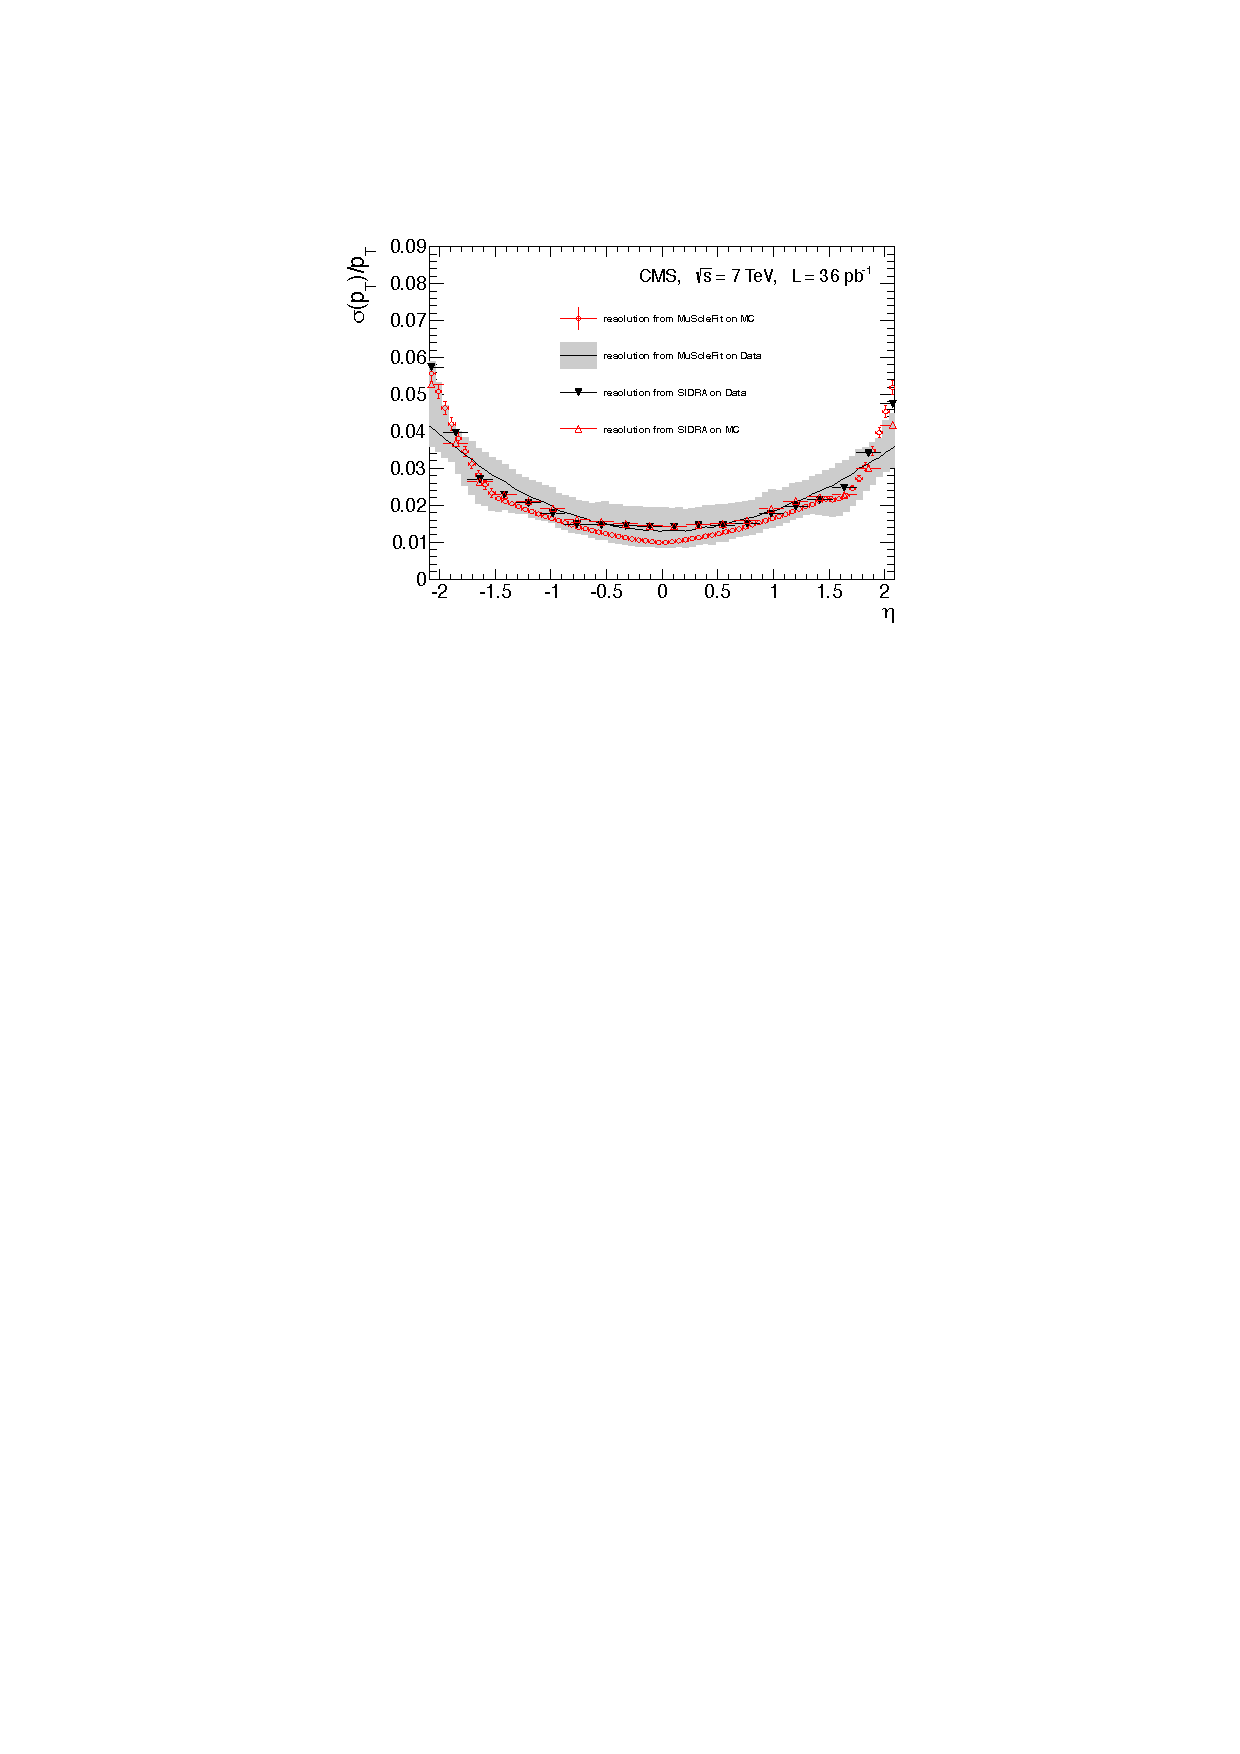
\includegraphics[width=5in]{figures/muonres.pdf}
\caption{Number of pileup vertices before and after reweighted is applied.}
\label{fig:pu}
\end{figure}

%The Summer16 Monte Carlo samples are reweighted  to match the pileup distribution in 2016 data. 
%The pileup weights are shown in Fig.~\ref{fig:PUrew} (right). They were computed from a Monte-Carlo pileup profile obtained directly from the 25ns 76X MC production parameter file, and a data pileup profile obtained using the rereco 50ns JSON file ($77\ \text{pb}^{-1}$) and the 25ns Silver JSON file ($2.63\ \text{fb}^{-1}$, taking $69\ \text{mb}^{-1}$). These profiles are shown in Fig.~\ref{fig:PUrew} (left).

%A closure test was performed with events preselected with the requirement of a Z candidate (Fig.~\ref{fig:PUrewtest}), showing a much better agreement in the distribution of the number of vertices when the reweighting is applied.
%The reweighting was found to increase the expected yield in the signal region by 0.4\%.


%=======
%\begin{figure}[!htb]
%\vspace*{0.3cm}
%\begin{center}
%\includegraphics[width=0.45\textwidth]{Figures/pileup76x50ns25nsSilver}
%\includegraphics[width=0.45\textwidth]{Figures/puweight76x50ns25nsSilver}
%\caption{(left) Data and Monte-Carlo pileup profiles that were used to compute the weights. (right) Pileup weights that are applied to simulation events.
%\label{fig:PUrew}}
%\end{center}
%\end{figure}
%=======

%=======
%\begin{figure}[!htb]
%\vspace*{0.3cm}
%\begin{center}
%\includegraphics[width=0.45\textwidth]{Figures/c_CheckPUReweighting_}
%\caption{Closure test: distribution of the number of vertices in simulation before and after reweighting compared to that in data, for a set of events containing a Z candidate as defined in Section~\ref{sec:zzcandsel}.
%\label{fig:PUrewtest}}
%\end{center}
%\end{figure}
%%=======

